\subsection{Overview}
In this last section we provide all the necessary specifications about the plan for the implementation and the testing of the system. This phase is, of course, critical for the development of a reliable software system. It is important to observe that, while testing can show the presence of bugs in the code, passing the tests does not imply the absence of errors in the final application. Still, with our tests, we will try to find the majority of the bugs before the product hits the market (and also after, maintenance is important).

\subsection{Implementation Plan}
For all the implementation processes we have chosen a \textbf{bottom-up} approach; %TODO
\\
The first element that we will implement is the \textbf{DBMSServices} component, which manages the model, i.e. the data, of our application, and so it is required by most of the components of the system.\\
After the data layer has been implemented we can proceed to the components that utilize it. The main logic of the application is implemented by the QueueManager component, so we would to implent it as soon as possible. In order to do this, we need to first realize the compoents on which the QueueManager depends. For this reason we will start by implementing \textbf{StatisticsManager}, and, in parallel, the \textbf{StoreMonitor}, then the \textbf{MonitorManager}.\\\\
At this point we have all the components needed for \textbf{QueueManager} to operate, so we implement it. Since almost all other components of the ApplicationServer rely on QueueManager and/or on DBMSServices to operate, we can now split our team to work in parallel on the following components: 
\begin{itemize}
	\item \textbf{AccessManager} composed of \textbf{LoginManager} and \textbf{SignUpManager}
	\item \textbf{UserManager} composed of \textbf{StoreOwnerManager} and \textbf{CustomerManager}
	\item \textbf{ReservationManager}
	\item \textbf{StoreManager}
	\item \textbf{QRManager}
	\item \textbf{PrinterManager}
	\item \textbf{NotificationManager}
\end{itemize}
After the creation of all these components, we can now create the element that routes the external queries to the various internal services: the \textbf{Redirector}.
Once this is done, all the modules required for the operation of the ApplicationServer have been implemented, so the application layer is completed. We can now proceed to realize the front end of the system.\\\\
First we work on the components that will run on the hardware interfaces of the stores, i.e. the \textbf{QRReader} and \textbf{TicketPrinter} (the StoreMonitor has already been implemented at the beginning). Then we realize the services that allow user interaction: \textbf{CustomerManager}, and \textbf{StoreOwnerService} in their respective versions for the \textbf{WebServer} and the SmartApp. The WebServer is complete, so we can instantiate the \textbf{WebApp}. For the SmartApp we also need the NotificationService which depends on \textbf{MapsAPI} to communicate with external mapping service (e.g. Google Maps). Therefore first we implement the latter, then the \textbf{NotificationService}, with which the \textbf{SmartApp} is complete.
\subsubsection{Integration Strategy}
For the implementation and testing plan we decided to use the \textbf{bottom-up} approach. According to this approach, we carry on the procedure as described in the following diagrams. 
\begin{figure}[H]
	\noindent
	\makebox[\textwidth]{ 
		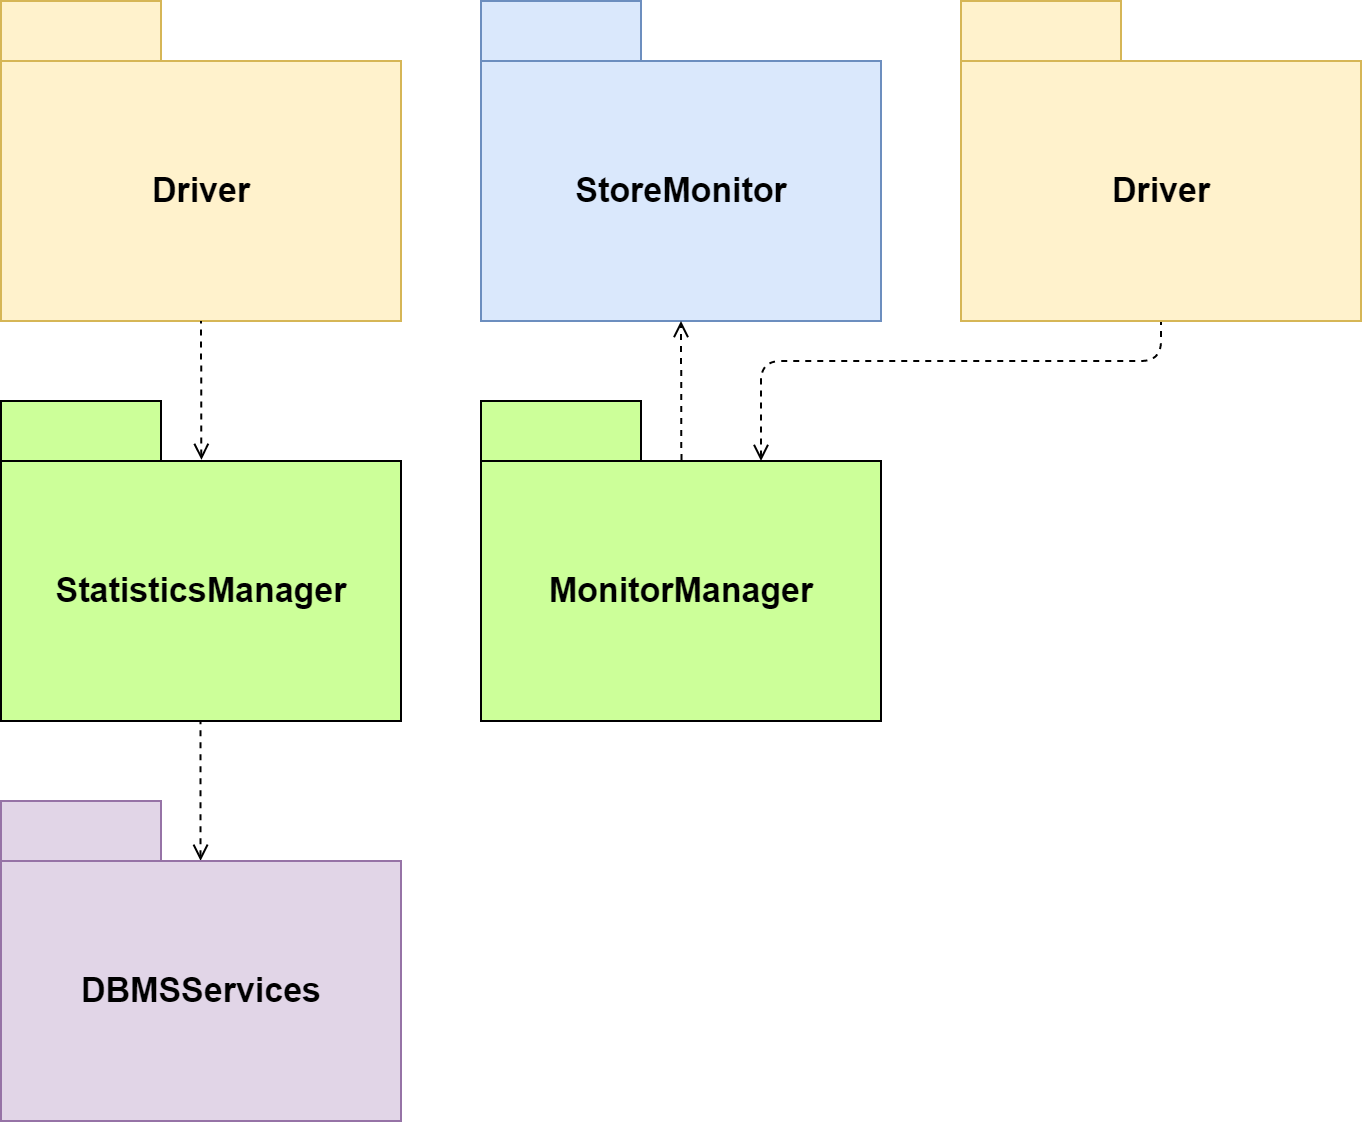
\includegraphics[scale=0.45]{Images/Test1.png}}
	\caption{Integration 1} %TODO: decide wether to keep captions
\end{figure}
The first element implemented and unit tested is the DBMSServices, followed by the components that will be necessary for the QueueManager, the core of the application. Of course the DBMSServices is the first to be implemented and tested because all other components rely on it in one way or another.
\begin{figure}[H]
	\noindent
	\makebox[\textwidth]{
		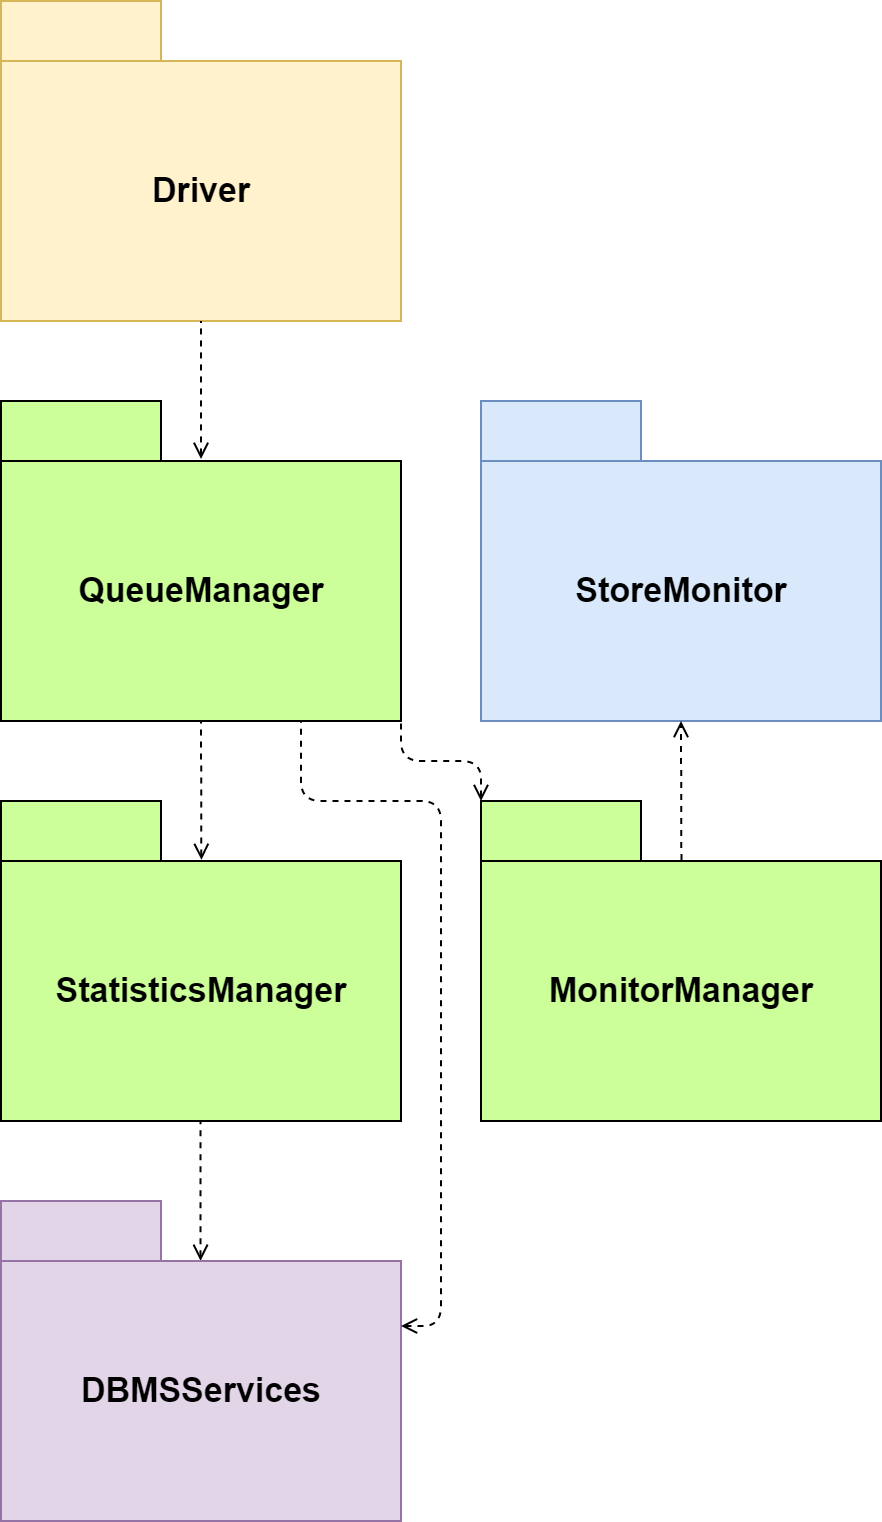
\includegraphics[scale=0.45]{Images/Test2.png}}
	\caption{Integration 2} %TODO: decide wether to keep captions
\end{figure}
The core of the system is now implemented and tested; it will be critical for most of the functionalities offered by the system: management of the reservation, QR, to notify customers with a smartphone app. The QueueManager relies on the components previously realized.
\begin{figure}[H]
	\noindent
	\makebox[\textwidth]{
		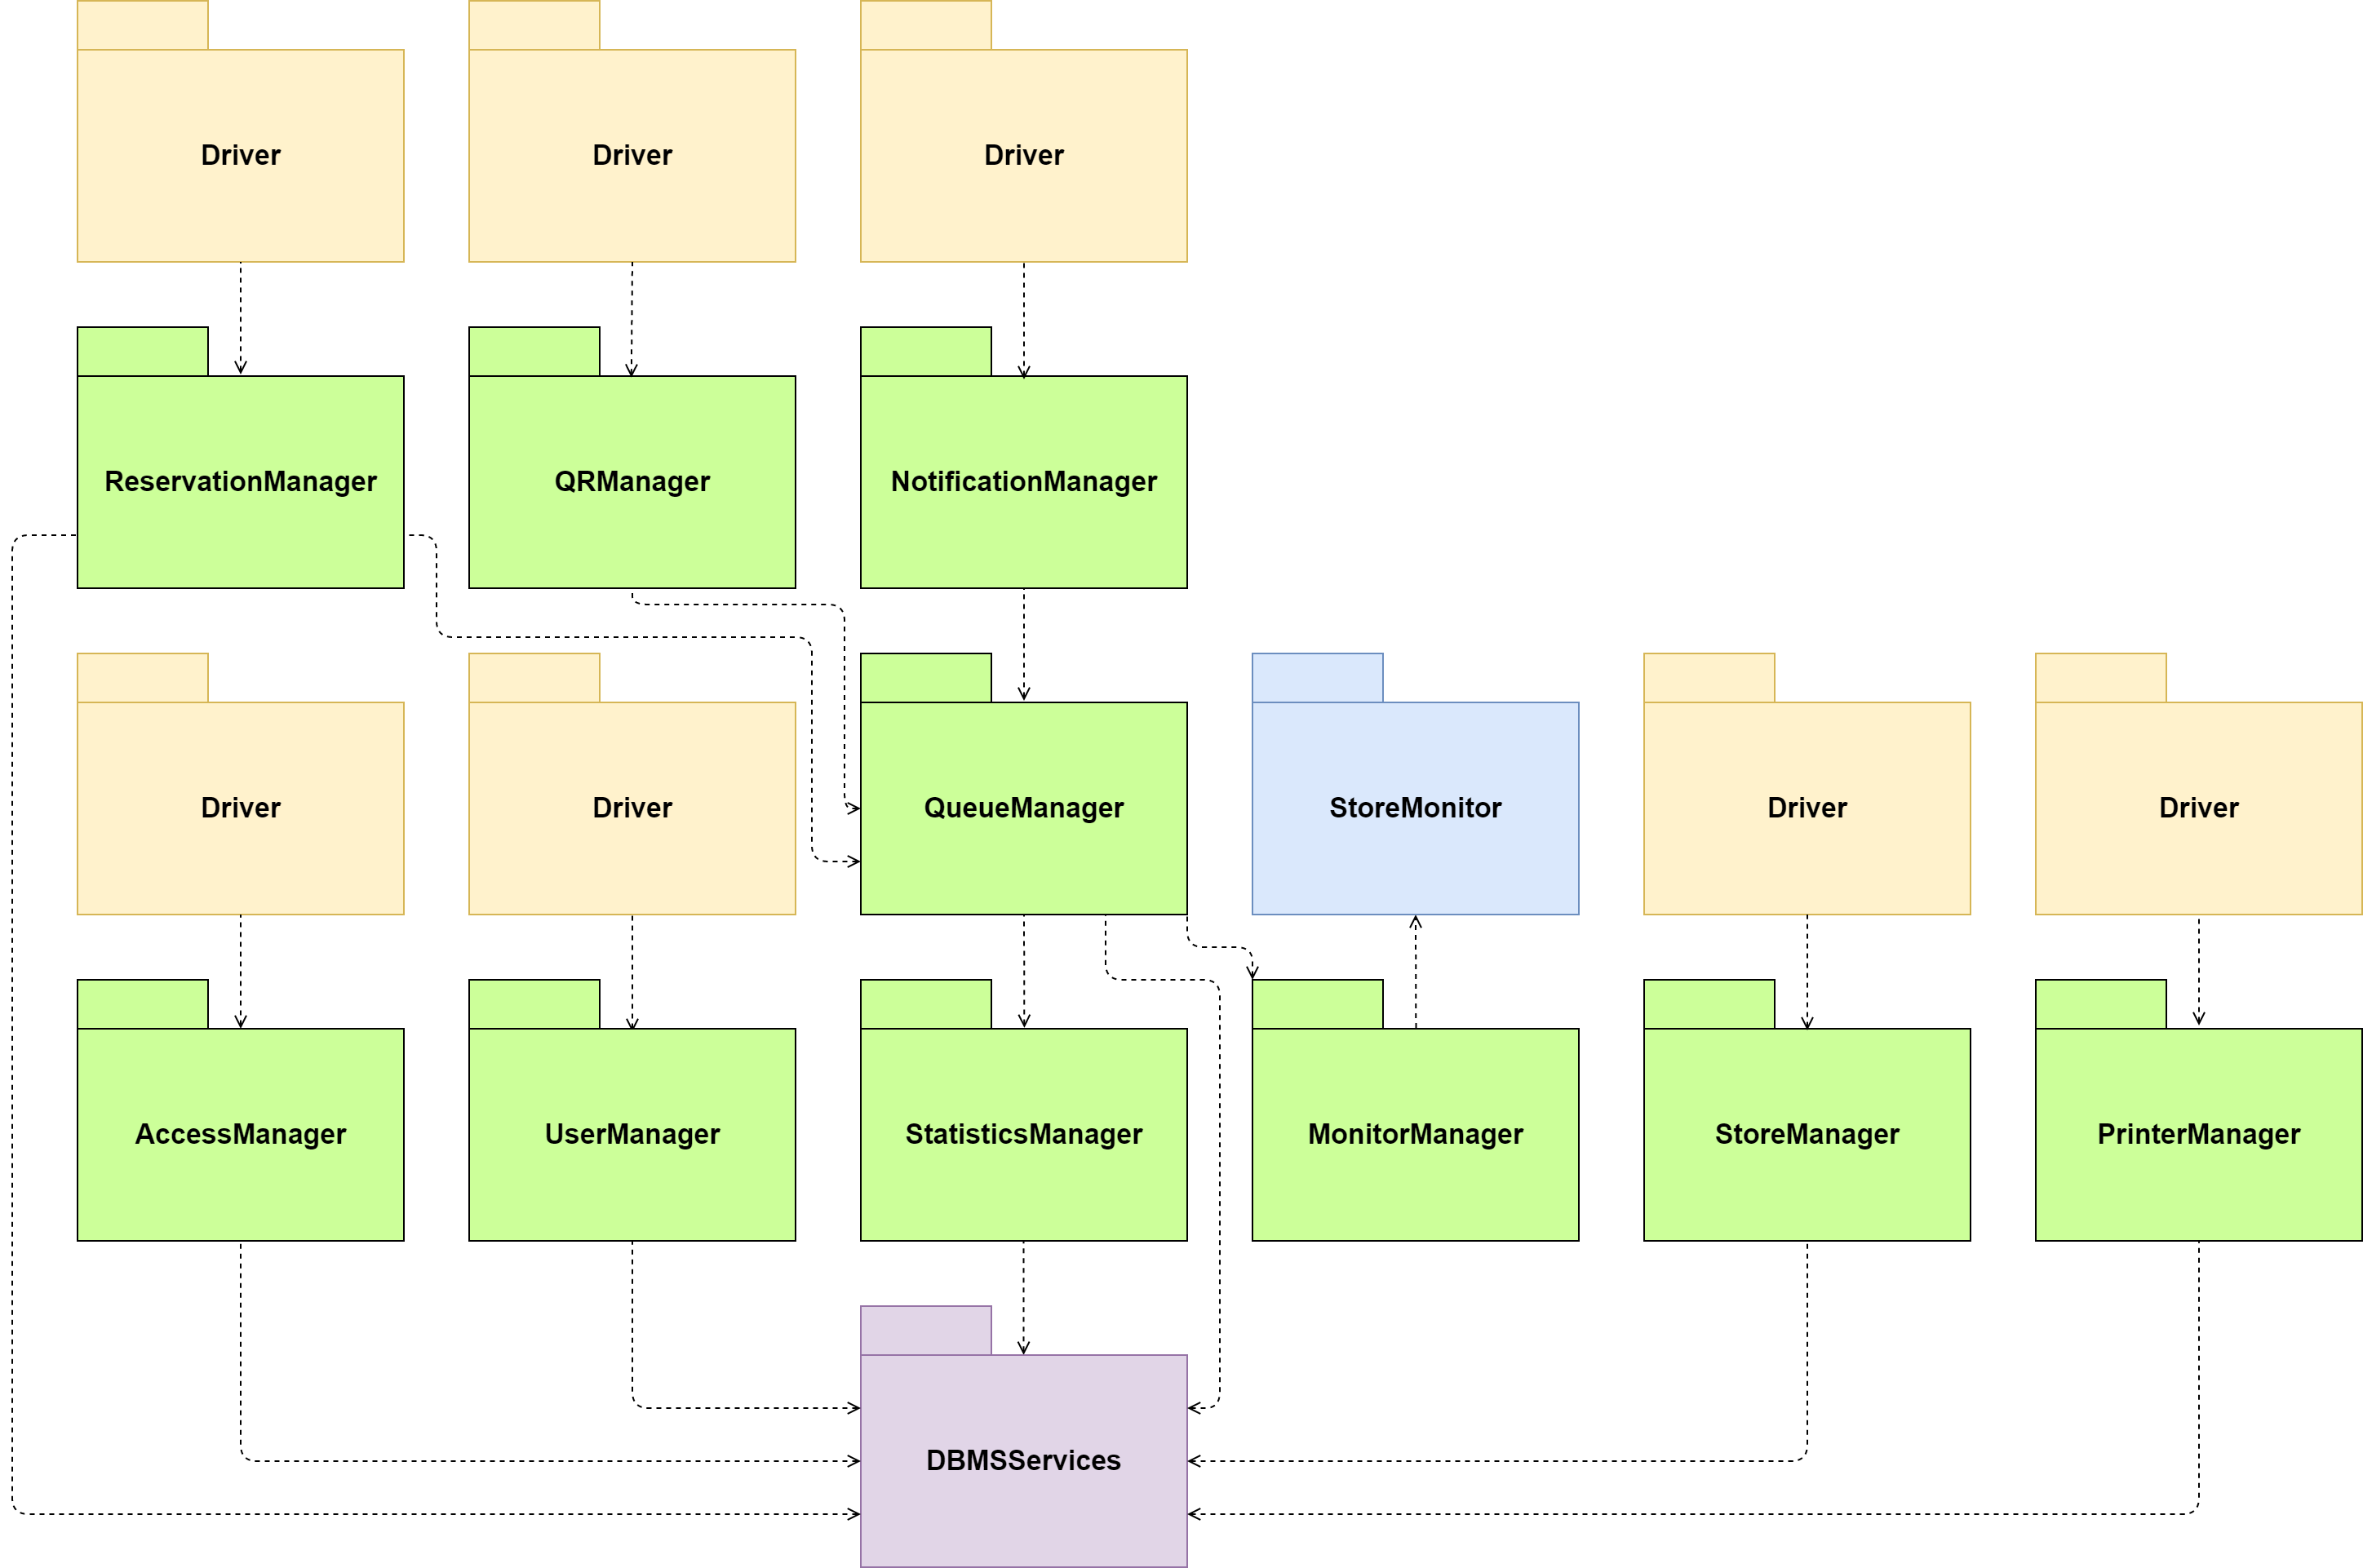
\includegraphics[scale=0.45]{Images/Test3.png}}
	\caption{Integration 3} %TODO: decide wether to keep captions
\end{figure}
Many components are implemented and unit tested in parallel and now they are integrated with the core of the system. The integration testing can now focus on most of the functionalities of the final system: log in, registration, management of user and store data, creation and deletion of reservations of different kind, QR generation and recognition, aggregation of data to build statistics, management of printers and monitors of each store. Of course each of these functionalities will need a driver in order to be tested. Moreover the parallelism can speed up the general development process.
\begin{figure}[H]
	\noindent
	\makebox[\textwidth]{
		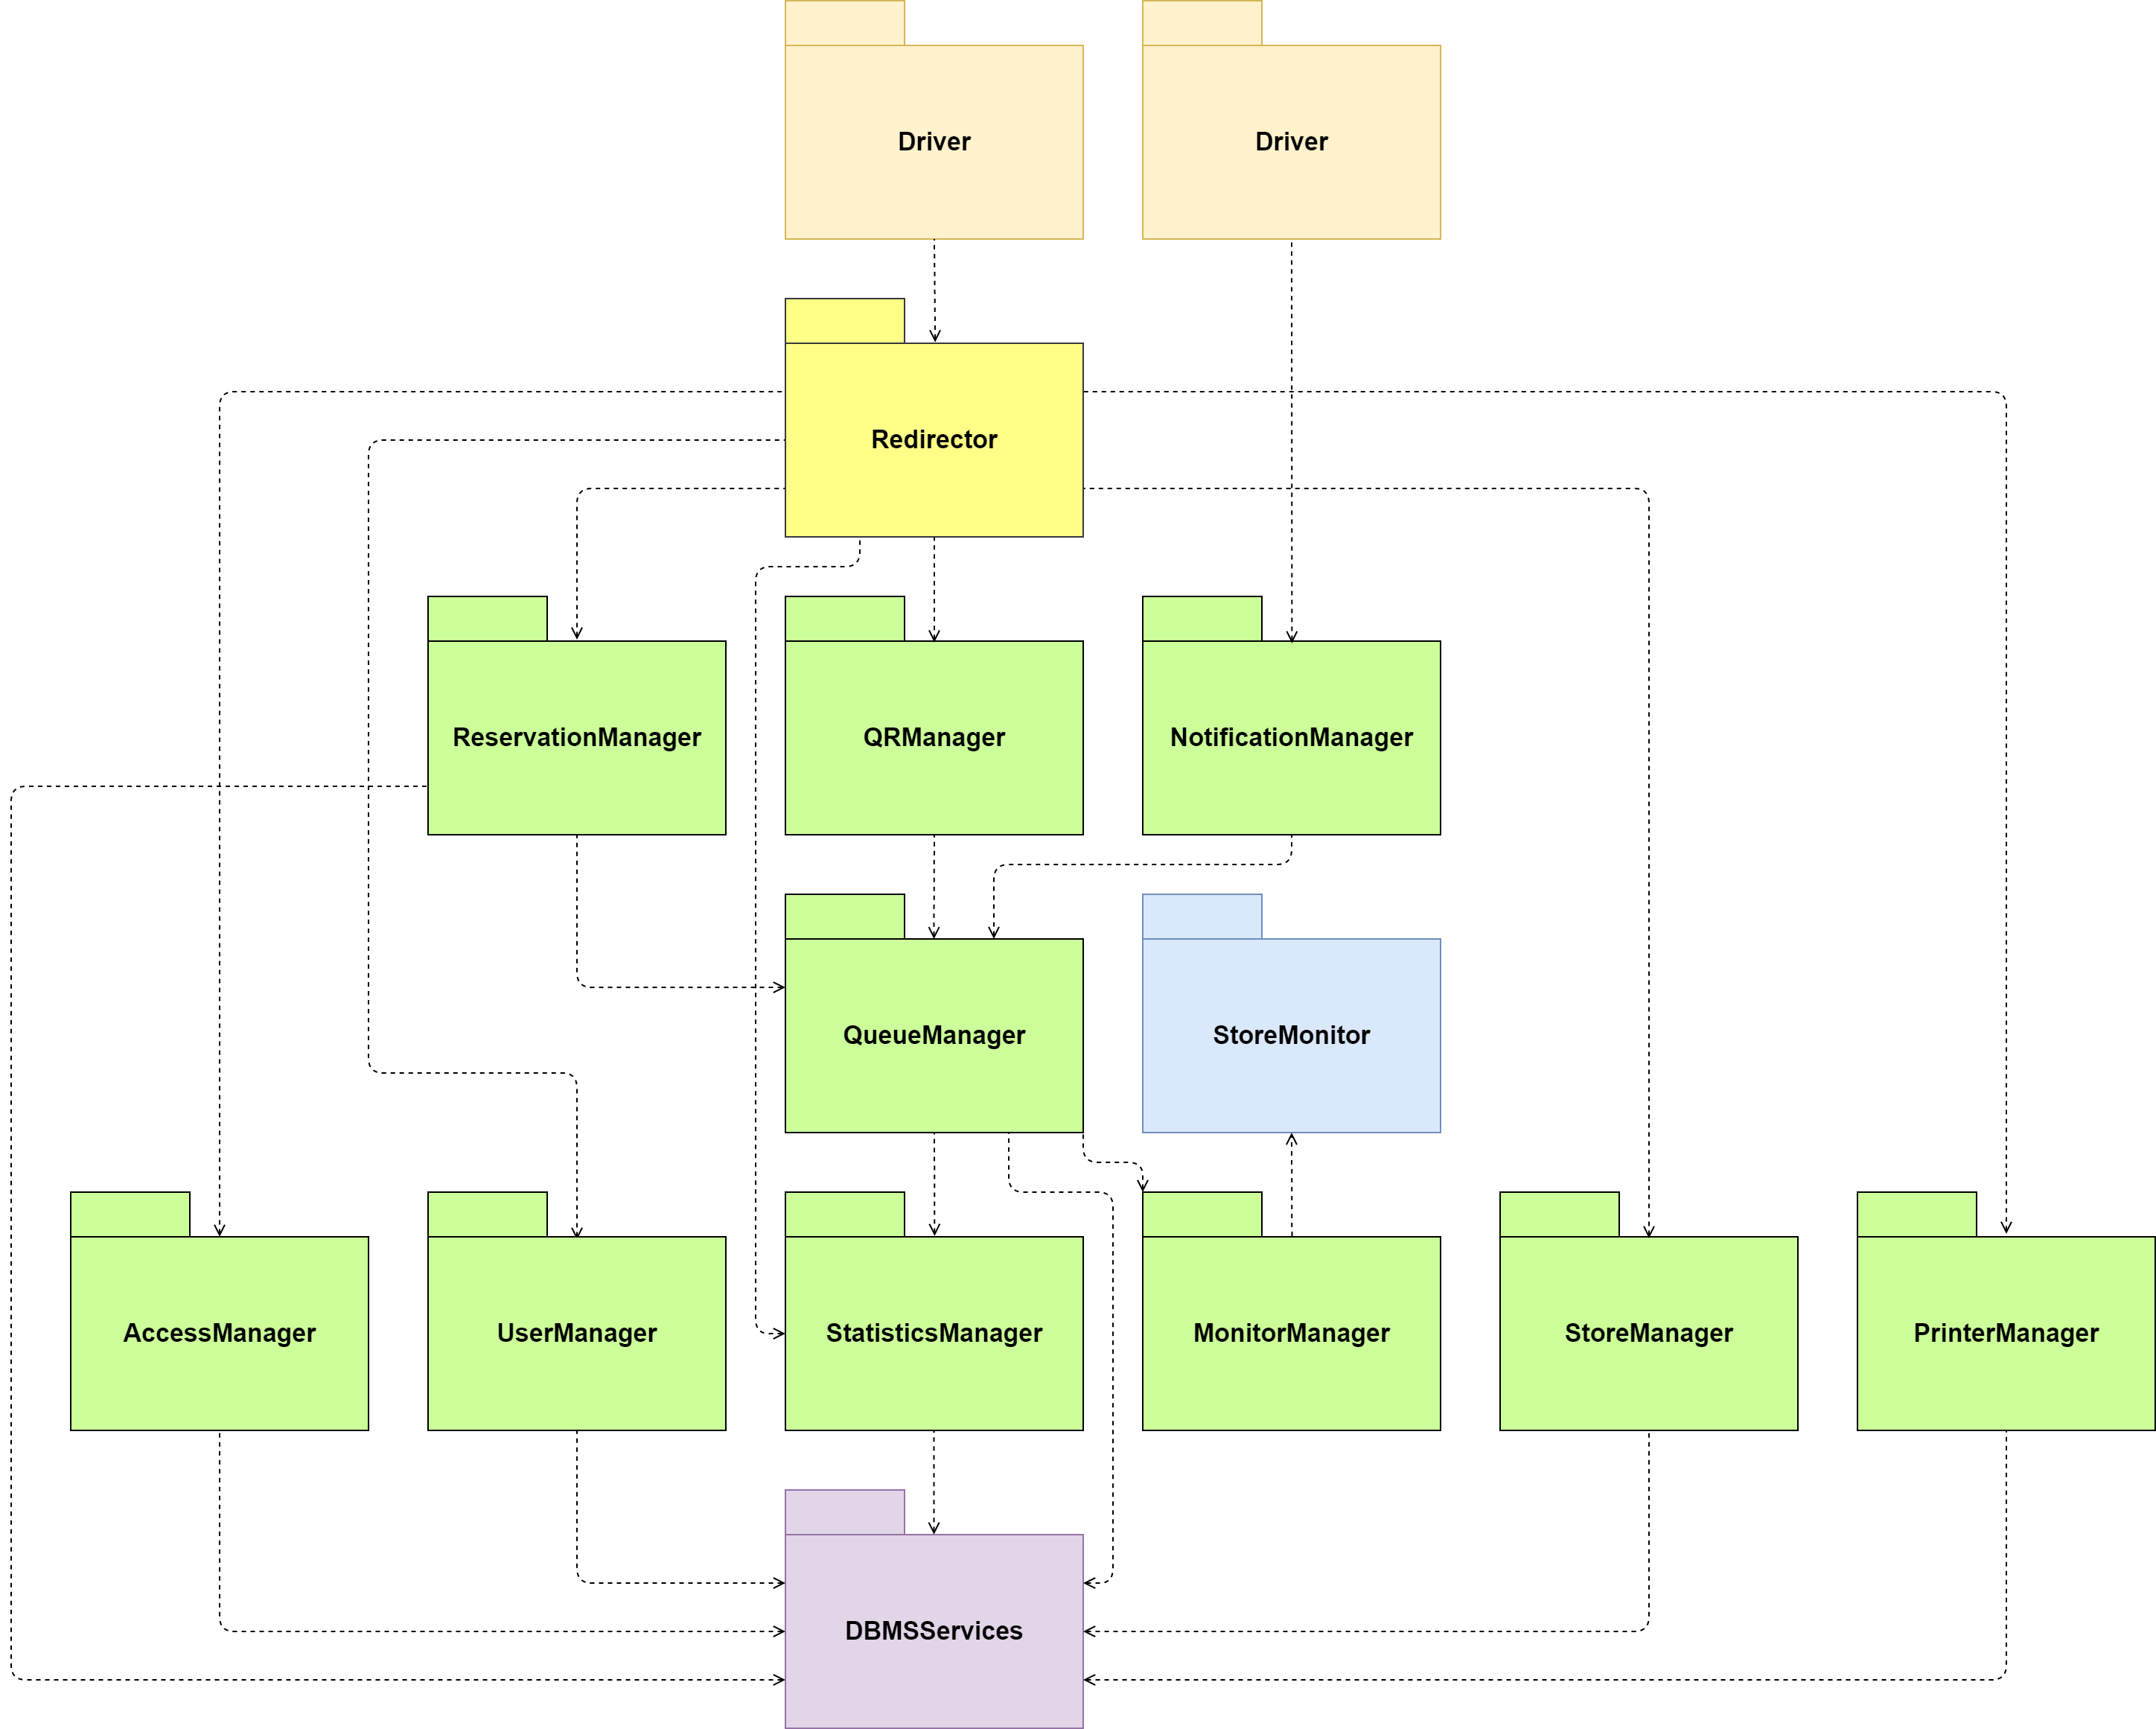
\includegraphics[scale=0.45]{Images/Test4.png}}
	\caption{Integration 4} %TODO: decide wether to keep captions
\end{figure}
The component that realizes the facade pattern, the redirector, is implemented, unit tested and integrated with the rest of the system. Obviously according to the bottom-up approach this component must be developed after all the other components on which it relies have been implemented. The NotificationManager still uses a Driver because it is not accessed directly from the Redirector. 
\begin{figure}[H]
	\noindent
	\makebox[\textwidth]{
		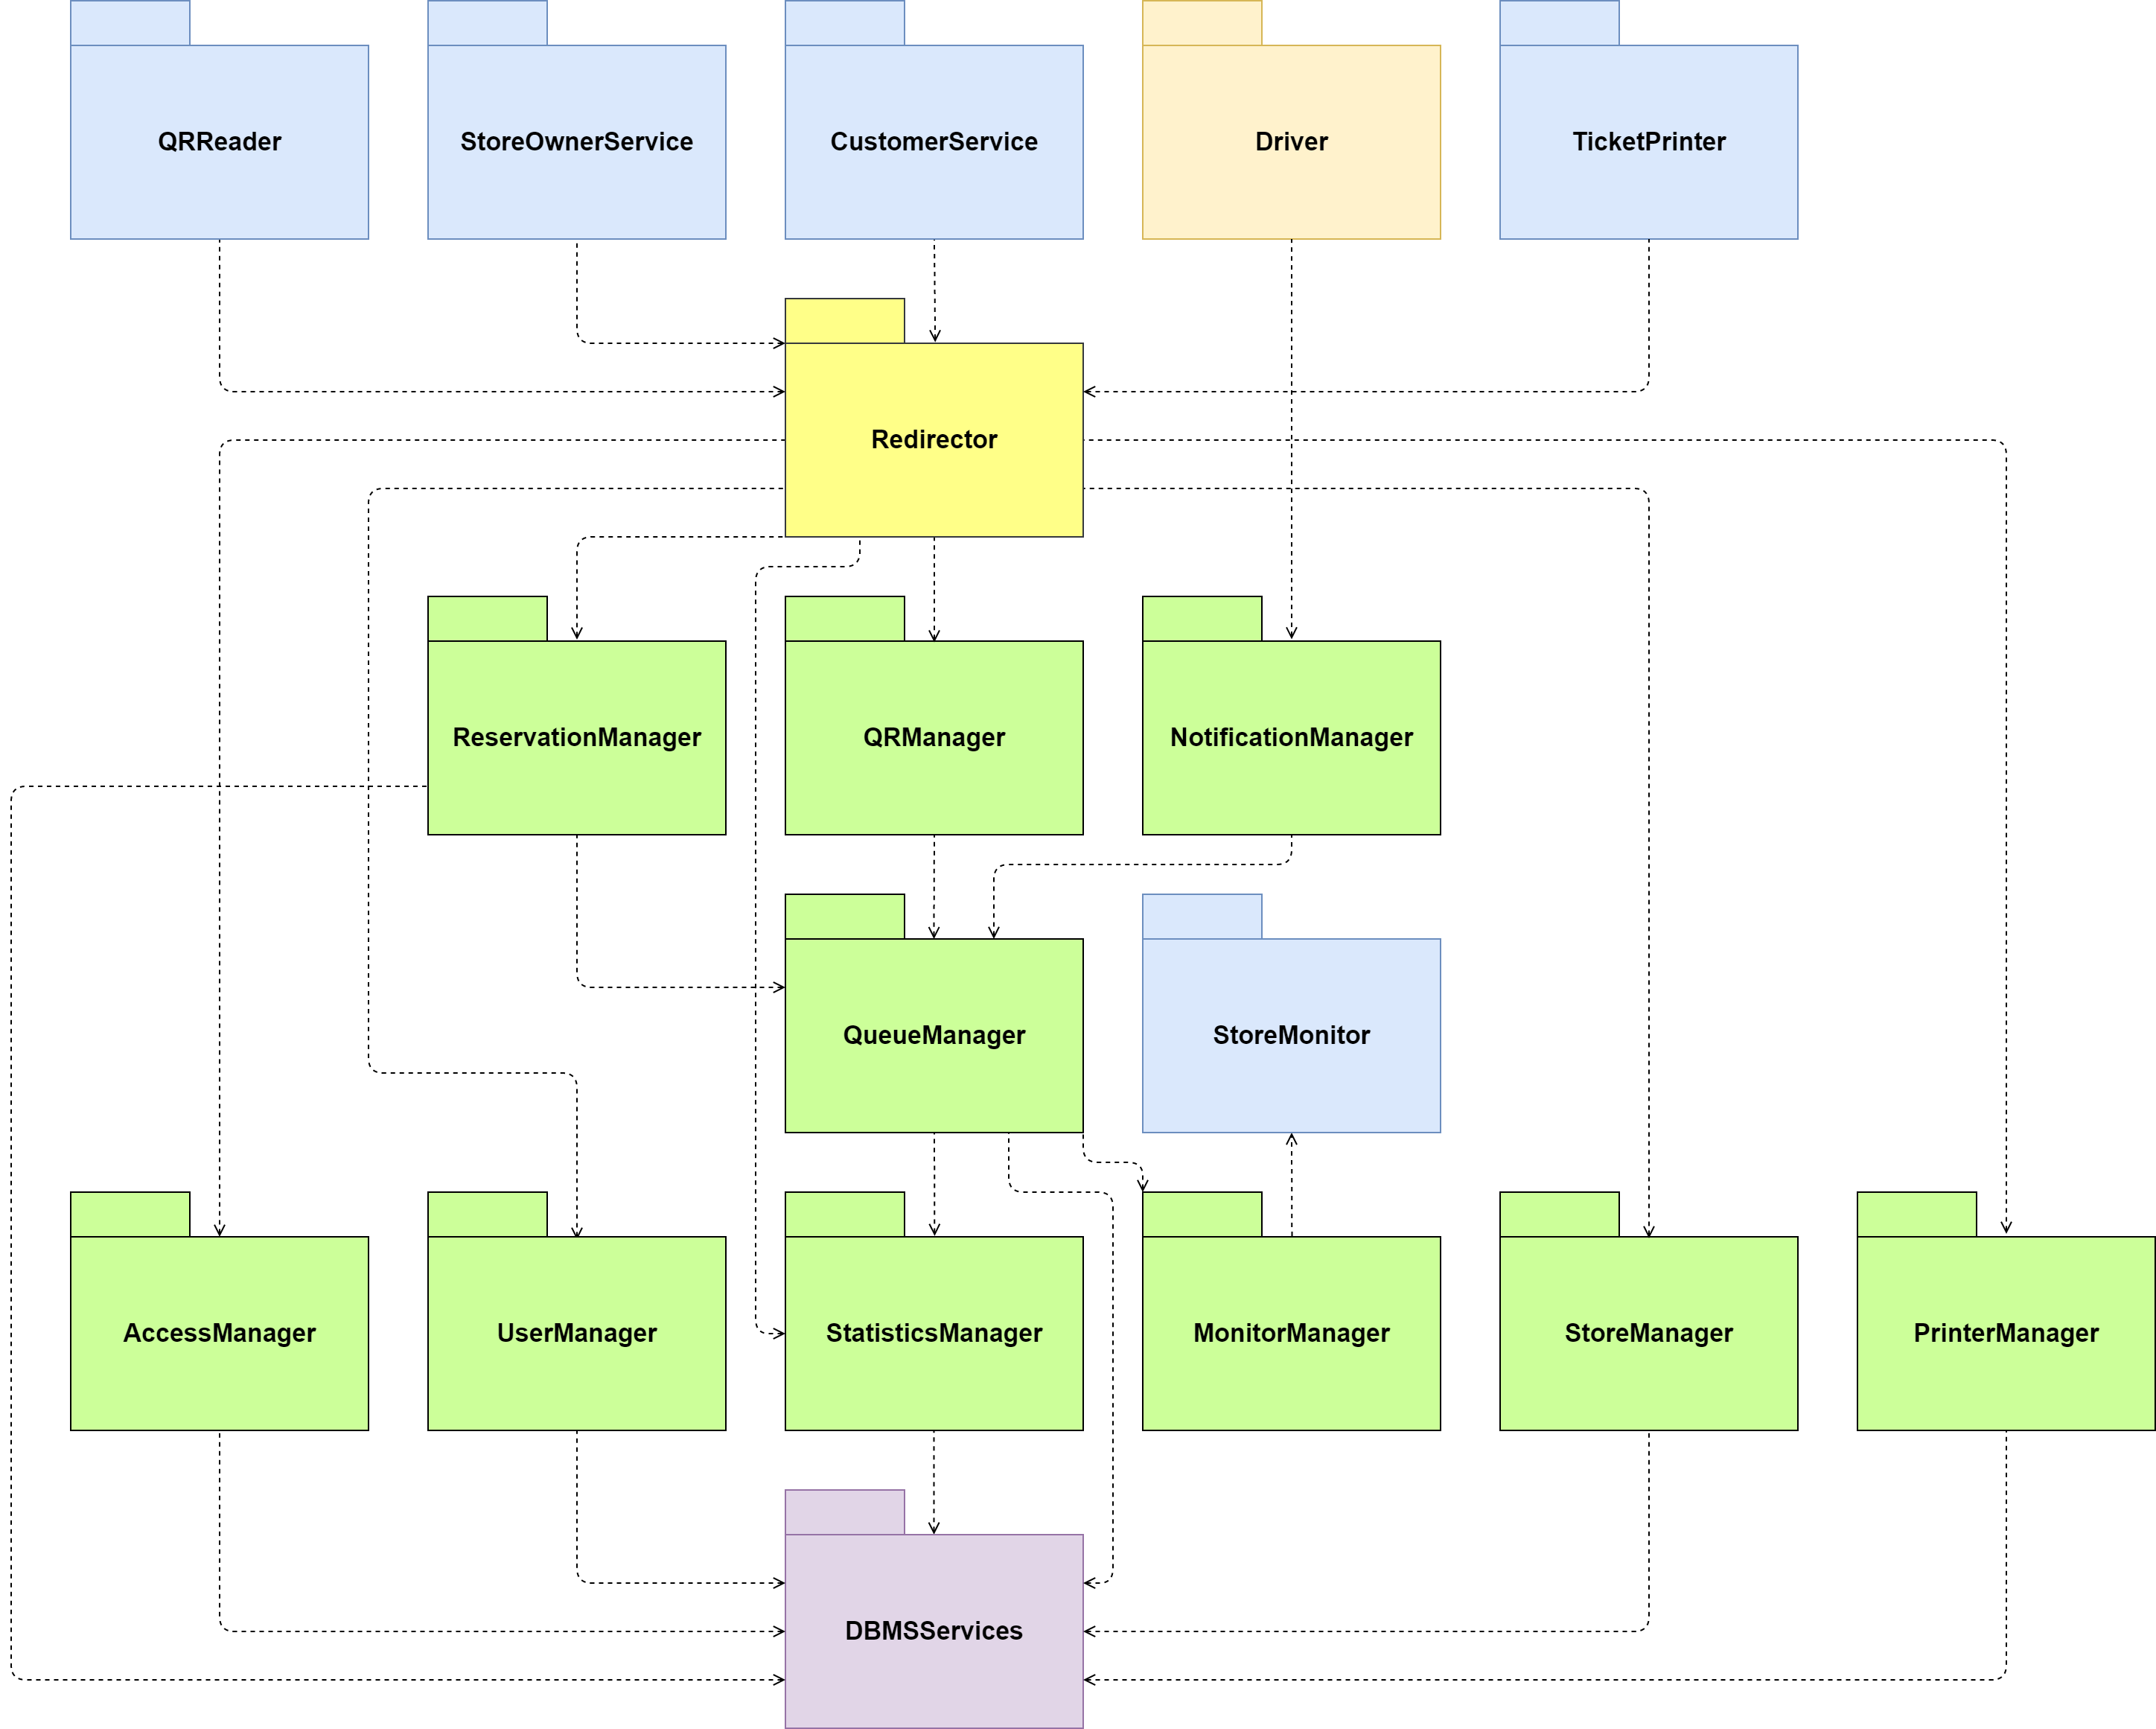
\includegraphics[scale=0.45]{Images/Test5.png}}
	\caption{Integration 5} %TODO: decide wether to keep captions
\end{figure}
At this step we implement and unit test in parallel the components that operate as interface between the system and the users: QRReader, StoreOwnerService, CustomerService and TicketPrinter have been added and integrated with the redirector.
\begin{figure}[H]
	\noindent
	\makebox[\textwidth]{
		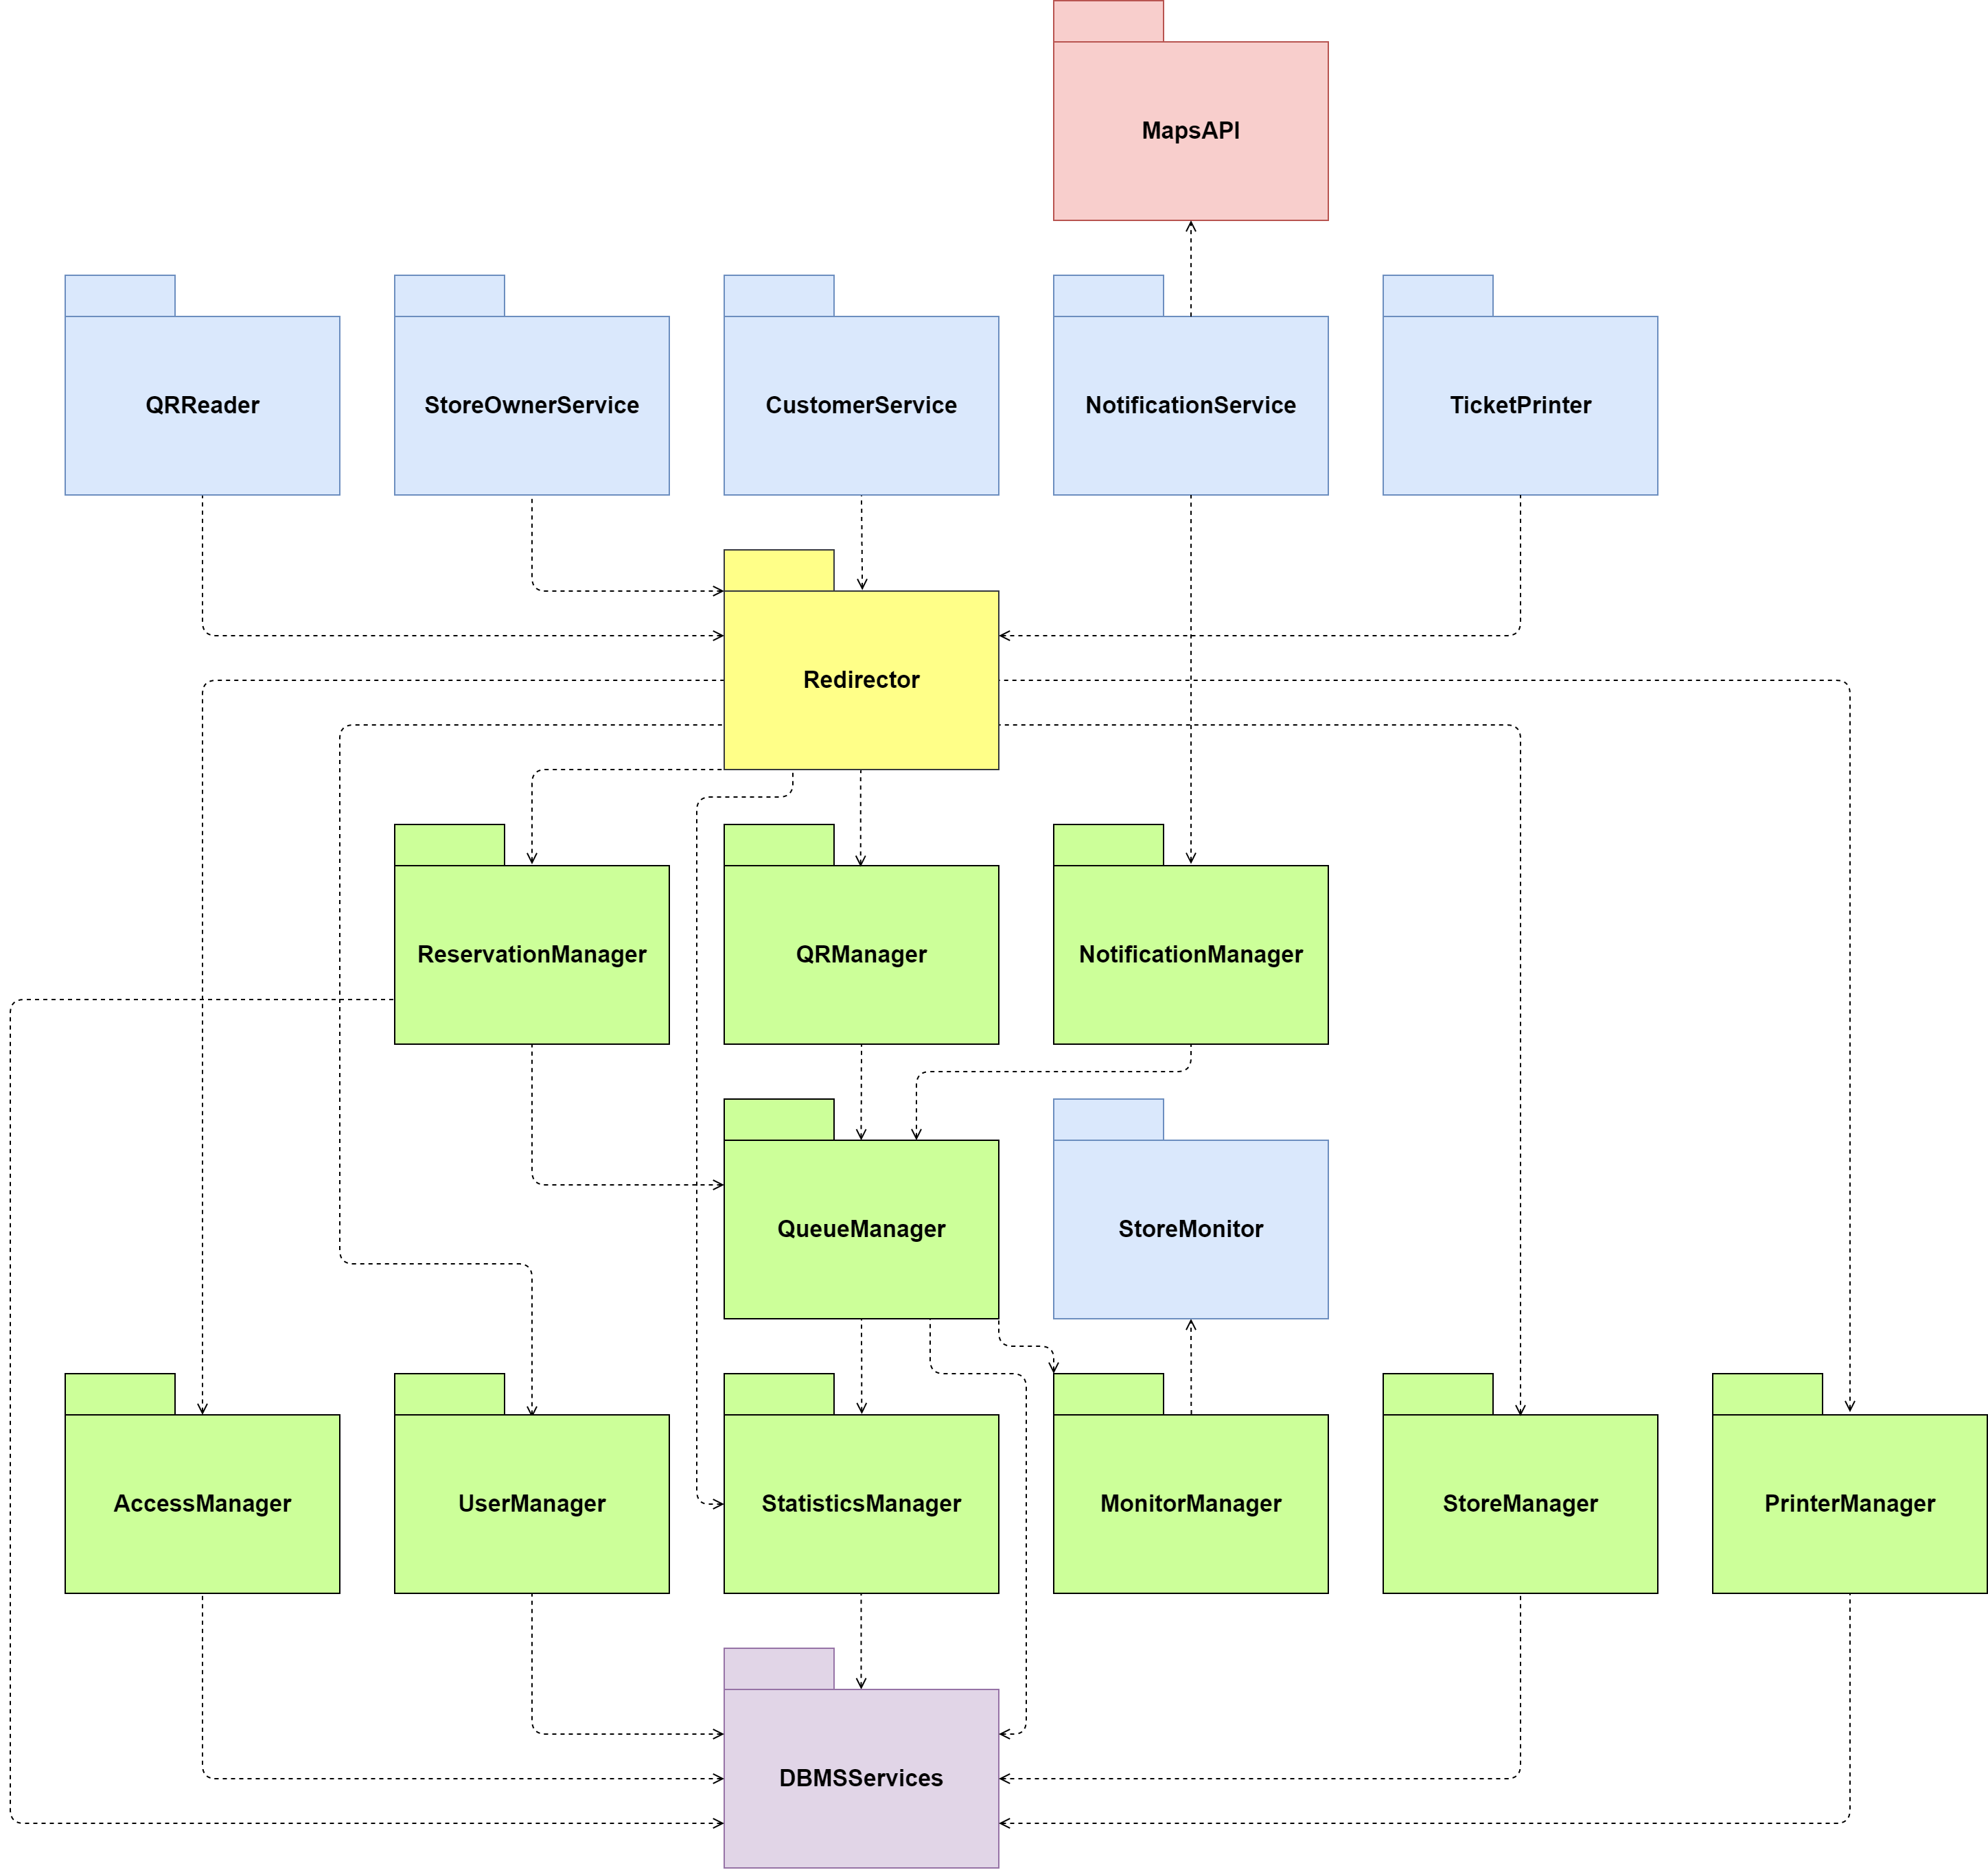
\includegraphics[scale=0.45]{Images/Test6.png}}
	\caption{Integration 6} %TODO: decide wether to keep captions
\end{figure}
Finally the last step is to develop the components that will enable the notification functionality for the customers. The NotificationService makes use of MapsAPI, which connects it with the external mapping service.\\\\
Now that every component of the system has been implemented and integrated we can proceed to the system testing phase.
\subsection{System Testing}
Onece the whole system has been developed we have to check that all functional and non functional requirements have been met. This is the purpose of the system testing. Note that testing environment should be as close as possible to deployment environment so as to give credibility to the results obtained. These tests will be carried out by an independent team with no knowledge of the internals of the system (black box testing).
System testing focuses not only on guaranteeing that all functionalities work as expected, but also on demonstrating the qualities of the application, through performance testing, stress testing and load testing.
\subsubsection{Performance testing}
Here we verify that the system matches expected performance requirements. This test will allow us to identify inefficient algorithms, bottlenecks, possibilities for query optimization as well as to produce a benchmark as a measure of the performance of the product, and to compare subsequent versions of the software.
\subsubsection{Load testing}
This phase aims to identify system behavior under heavy load conditions. Here we try to load the system until we reach its theoretical threshold and observe how and how long it manages to work without failing. This test's purpose is to find memory leaks, excessive use of memory, and buffer overflows.
\subsubsection{Stress testing}
In this phase we overload the system and observe how the system recovers from failure. We would like that the application could come back on line gracefully.
\subsection{Additional testing specifications}